\documentclass{beamer}
\usepackage{graphicx, color}

% Use something like:
% % Use something like:
% % Use something like:
% \input{../../macros}

% groupings of objects.
\newcommand{\set}[1]{\ensuremath{\left\{ #1 \right\}}}
\newcommand{\seq}[1]{\ensuremath{\left(#1\right)}}
\newcommand{\ang}[1]{\ensuremath{\langle#1\rangle}}
\newcommand{\tuple}[1]{\ensuremath{\left(#1\right)}}
\newcommand{\size}[1]{\ensuremath{\left| #1\right|}}

% numerical shortcuts.
\newcommand{\abs}[1]{\ensuremath{\left| #1\right|}}
\newcommand{\floor}[1]{\ensuremath{\left\lfloor #1 \right\rfloor}}
\newcommand{\ceil}[1]{\ensuremath{\left\lceil #1 \right\rceil}}

% linear algebra shortcuts.
\newcommand{\change}{\ensuremath{\Delta}}
\newcommand{\norm}[1]{\ensuremath{\left\| #1\right\|}}
\newcommand{\dprod}[1]{\ensuremath{\langle#1\rangle}}
\newcommand{\linspan}[1]{\ensuremath{\langle#1\rangle}}
\newcommand{\conj}[1]{\ensuremath{\overline{#1}}}
\newcommand{\der}{\ensuremath{\frac{d}{dx}}}
\newcommand{\lap}{\ensuremath{\Delta}}
\newcommand{\kron}{\ensuremath{\otimes}}
\newcommand{\nperp}{\ensuremath{\nvdash}}

\newcommand{\mat}[1]{\left[ \begin{smallmatrix}#1 \end{smallmatrix} \right]}

% derivatives and limits
\newcommand{\partder}[2]{\ensuremath{\frac{\partial #1}{\partial #2}}}
\newcommand{\partdern}[3]{\ensuremath{\frac{\partial^{#3} #1}{\partial #2^{#3}}}}
\newcommand{\gradient}{\ensuremath{\nabla}}
\newcommand{\subdifferential}{\ensuremath{\partial}}

% Arrows
\newcommand{\diverge}{\ensuremath{\nearrow}}
\newcommand{\notto}{\ensuremath{\nrightarrow}}
\newcommand{\up}{\ensuremath{\uparrow}}
\newcommand{\down}{\ensuremath{\downarrow}}
% gets and gives are defined!

% ordering operators
\newcommand{\oleq}{\preceq}
\newcommand{\ogeq}{\succeq}

% programming and logic operators
\newcommand{\dfn}{:=}
\newcommand{\assign}{:=}
\newcommand{\co}{\ co\ }
\newcommand{\en}{\ en\ }


% logic operators
\newcommand{\xor}{\ensuremath{\oplus}}
\newcommand{\Land}{\ensuremath{\bigwedge}}
\newcommand{\Lor}{\ensuremath{\bigvee}}
\newcommand{\finish}{\ensuremath{\Box}}
\newcommand{\contra}{\ensuremath{\Rightarrow \Leftarrow}}
\newcommand{\iseq}{\ensuremath{\stackrel{_?}{=}}}


% Set theory
\newcommand{\symdiff}{\ensuremath{\Delta}}
\newcommand{\union}{\ensuremath{\cup}}
\newcommand{\inters}{\ensuremath{\cap}}
\newcommand{\Union}{\ensuremath{\bigcup}}
\newcommand{\Inters}{\ensuremath{\bigcap}}
\newcommand{\nullSet}{\ensuremath{\phi}}


% graph theory
\newcommand{\nbd}{\Gamma}

% Script alphabets
% For reals, use \Re

% greek letters
\newcommand{\eps}{\ensuremath{\epsilon}}
\newcommand{\del}{\ensuremath{\delta}}
\newcommand{\ga}{\ensuremath{\alpha}}
\newcommand{\gb}{\ensuremath{\beta}}
\newcommand{\gd}{\ensuremath{\del}}
\newcommand{\gp}{\ensuremath{\pi}}
\newcommand{\gf}{\ensuremath{\phi}}
\newcommand{\gh}{\ensuremath{\eta}}
\newcommand{\gF}{\ensuremath{\Phi}}
\newcommand{\gl}{\ensuremath{\lambda}}
\newcommand{\gm}{\ensuremath{\mu}}
\newcommand{\gn}{\ensuremath{\nu}}
\newcommand{\gr}{\ensuremath{\rho}}
\newcommand{\gs}{\ensuremath{\sigma}}
\newcommand{\gt}{\ensuremath{\theta}}
\newcommand{\gx}{\ensuremath{\xi}}

\newcommand{\sw}{\ensuremath{\sigma}}
\newcommand{\SW}{\ensuremath{\Sigma}}
\newcommand{\ew}{\ensuremath{\lambda}}
\newcommand{\EW}{\ensuremath{\Lambda}}

\newcommand{\Del}{\ensuremath{\Delta}}
\newcommand{\gD}{\ensuremath{\Delta}}
\newcommand{\gG}{\ensuremath{\Gamma}}
\newcommand{\gO}{\ensuremath{\Omega}}
\newcommand{\gS}{\ensuremath{\Sigma}}

% Bold english letters.
\newcommand{\bA}{\ensuremath{\mathbf{A}}}
\newcommand{\bB}{\ensuremath{\mathbf{B}}}
\newcommand{\bC}{\ensuremath{\mathbf{C}}}
\newcommand{\bD}{\ensuremath{\mathbf{D}}}
\newcommand{\bE}{\ensuremath{\mathbf{E}}}
\newcommand{\bF}{\ensuremath{\mathbf{F}}}
\newcommand{\bG}{\ensuremath{\mathbf{G}}}
\newcommand{\bH}{\ensuremath{\mathbf{H}}}
\newcommand{\bI}{\ensuremath{\mathbf{I}}}
\newcommand{\bJ}{\ensuremath{\mathbf{J}}}
\newcommand{\bK}{\ensuremath{\mathbf{K}}}
\newcommand{\bL}{\ensuremath{\mathbf{L}}}
\newcommand{\bM}{\ensuremath{\mathbf{M}}}
\newcommand{\bN}{\ensuremath{\mathbf{N}}}
\newcommand{\bO}{\ensuremath{\mathbf{O}}}
\newcommand{\bP}{\ensuremath{\mathbf{P}}}
\newcommand{\bQ}{\ensuremath{\mathbf{Q}}}
\newcommand{\bR}{\ensuremath{\mathbf{R}}} % PROSPER defines \R
\newcommand{\bS}{\ensuremath{\mathbf{S}}}
\newcommand{\bT}{\ensuremath{\mathbf{T}}}
\newcommand{\bU}{\ensuremath{\mathbf{U}}}
\newcommand{\bV}{\ensuremath{\mathbf{V}}}
\newcommand{\bW}{\ensuremath{\mathbf{W}}}
\newcommand{\bX}{\ensuremath{\mathbf{X}}}
\newcommand{\bY}{\ensuremath{\mathbf{Y}}}
\newcommand{\bZ}{\ensuremath{\mathbf{Z}}}
\newcommand{\bba}{\ensuremath{\mathbf{a}}}
\newcommand{\bbb}{\ensuremath{\mathbf{b}}}
\newcommand{\bbc}{\ensuremath{\mathbf{c}}}
\newcommand{\bbd}{\ensuremath{\mathbf{d}}}
\newcommand{\bbe}{\ensuremath{\mathbf{e}}}
\newcommand{\bbf}{\ensuremath{\mathbf{f}}}
\newcommand{\bbg}{\ensuremath{\mathbf{g}}}
\newcommand{\bbh}{\ensuremath{\mathbf{h}}}
\newcommand{\bbk}{\ensuremath{\mathbf{k}}}
\newcommand{\bbl}{\ensuremath{\mathbf{l}}}
\newcommand{\bbm}{\ensuremath{\mathbf{m}}}
\newcommand{\bbn}{\ensuremath{\mathbf{n}}}
\newcommand{\bbp}{\ensuremath{\mathbf{p}}}
\newcommand{\bbq}{\ensuremath{\mathbf{q}}}
\newcommand{\bbr}{\ensuremath{\mathbf{r}}}
\newcommand{\bbs}{\ensuremath{\mathbf{s}}}  % TIPA defines \s and LaTeX \ss!
\newcommand{\bbt}{\ensuremath{\mathbf{t}}}
\newcommand{\bbu}{\ensuremath{\mathbf{u}}}
\newcommand{\bbv}{\ensuremath{\mathbf{v}}}
\newcommand{\bbw}{\ensuremath{\mathbf{w}}}
\newcommand{\bbx}{\ensuremath{\mathbf{x}}}
\newcommand{\bby}{\ensuremath{\mathbf{y}}}
\newcommand{\bbz}{\ensuremath{\mathbf{z}}}
\newcommand{\0}{\ensuremath{\mathbf{0}}}
\newcommand{\1}{\ensuremath{\mathbf{1}}}


% Formatting shortcuts
\newcommand{\red}[1]{\textcolor{red}{#1}}
\newcommand{\green}[1]{\textcolor{green}{#1}}
\newcommand{\magenta}[1]{\textcolor{magenta}{#1}}
\newcommand{\orange}[1]{\textcolor{orange}{#1}}
\newcommand{\gray}[1]{\textcolor{gray}{#1}}
\newcommand{\blue}[1]{\textcolor{blue}{#1}}
\newcommand{\htext}[2]{\texorpdfstring{#1}{#2}}

% Statistics
\newcommand{\distr}{\ensuremath{\sim}}
\newcommand{\stddev}{\ensuremath{\sigma}}
\newcommand{\covmatrix}{\ensuremath{\Sigma}}
\newcommand{\mean}{\ensuremath{\mu}}
\newcommand{\param}{\ensuremath{\gt}}
\newcommand{\ftr}{\ensuremath{\phi}}

% General utility
\newcommand{\todo}[1]{\textbf{[TODO]}] \footnote{TODO: #1}}
\newcommand{\exclaim}[1]{{\textbf{\textit{#1}}}}
\newcommand{\tbc}{[\textbf{Incomplete}]}
\newcommand{\chk}{[\textbf{Check}]}
\newcommand{\oprob}{[\textbf{OP}]:}
\newcommand{\core}[1]{\textbf{Core Idea:}}
\newcommand{\why}{[\textbf{Find proof}]}
\newcommand{\opt}[1]{\textit{#1}}


\renewcommand{\~}{\htext{$\sim$}{~}}

\DeclareMathOperator*{\argmin}{arg\,min}
\DeclareMathOperator*{\argmax}{arg\,max}

% Items pertaining to the headed list.
\newcommand{\headeditem}[1]{\item\textbf{#1}}
\newcommand{\headedsubitem}[1]{\subitem\textbf{#1}}



% groupings of objects.
\newcommand{\set}[1]{\ensuremath{\left\{ #1 \right\}}}
\newcommand{\seq}[1]{\ensuremath{\left(#1\right)}}
\newcommand{\ang}[1]{\ensuremath{\langle#1\rangle}}
\newcommand{\tuple}[1]{\ensuremath{\left(#1\right)}}
\newcommand{\size}[1]{\ensuremath{\left| #1\right|}}

% numerical shortcuts.
\newcommand{\abs}[1]{\ensuremath{\left| #1\right|}}
\newcommand{\floor}[1]{\ensuremath{\left\lfloor #1 \right\rfloor}}
\newcommand{\ceil}[1]{\ensuremath{\left\lceil #1 \right\rceil}}

% linear algebra shortcuts.
\newcommand{\change}{\ensuremath{\Delta}}
\newcommand{\norm}[1]{\ensuremath{\left\| #1\right\|}}
\newcommand{\dprod}[1]{\ensuremath{\langle#1\rangle}}
\newcommand{\linspan}[1]{\ensuremath{\langle#1\rangle}}
\newcommand{\conj}[1]{\ensuremath{\overline{#1}}}
\newcommand{\der}{\ensuremath{\frac{d}{dx}}}
\newcommand{\lap}{\ensuremath{\Delta}}
\newcommand{\kron}{\ensuremath{\otimes}}
\newcommand{\nperp}{\ensuremath{\nvdash}}

\newcommand{\mat}[1]{\left[ \begin{smallmatrix}#1 \end{smallmatrix} \right]}

% derivatives and limits
\newcommand{\partder}[2]{\ensuremath{\frac{\partial #1}{\partial #2}}}
\newcommand{\partdern}[3]{\ensuremath{\frac{\partial^{#3} #1}{\partial #2^{#3}}}}
\newcommand{\gradient}{\ensuremath{\nabla}}
\newcommand{\subdifferential}{\ensuremath{\partial}}

% Arrows
\newcommand{\diverge}{\ensuremath{\nearrow}}
\newcommand{\notto}{\ensuremath{\nrightarrow}}
\newcommand{\up}{\ensuremath{\uparrow}}
\newcommand{\down}{\ensuremath{\downarrow}}
% gets and gives are defined!

% ordering operators
\newcommand{\oleq}{\preceq}
\newcommand{\ogeq}{\succeq}

% programming and logic operators
\newcommand{\dfn}{:=}
\newcommand{\assign}{:=}
\newcommand{\co}{\ co\ }
\newcommand{\en}{\ en\ }


% logic operators
\newcommand{\xor}{\ensuremath{\oplus}}
\newcommand{\Land}{\ensuremath{\bigwedge}}
\newcommand{\Lor}{\ensuremath{\bigvee}}
\newcommand{\finish}{\ensuremath{\Box}}
\newcommand{\contra}{\ensuremath{\Rightarrow \Leftarrow}}
\newcommand{\iseq}{\ensuremath{\stackrel{_?}{=}}}


% Set theory
\newcommand{\symdiff}{\ensuremath{\Delta}}
\newcommand{\union}{\ensuremath{\cup}}
\newcommand{\inters}{\ensuremath{\cap}}
\newcommand{\Union}{\ensuremath{\bigcup}}
\newcommand{\Inters}{\ensuremath{\bigcap}}
\newcommand{\nullSet}{\ensuremath{\phi}}


% graph theory
\newcommand{\nbd}{\Gamma}

% Script alphabets
% For reals, use \Re

% greek letters
\newcommand{\eps}{\ensuremath{\epsilon}}
\newcommand{\del}{\ensuremath{\delta}}
\newcommand{\ga}{\ensuremath{\alpha}}
\newcommand{\gb}{\ensuremath{\beta}}
\newcommand{\gd}{\ensuremath{\del}}
\newcommand{\gp}{\ensuremath{\pi}}
\newcommand{\gf}{\ensuremath{\phi}}
\newcommand{\gh}{\ensuremath{\eta}}
\newcommand{\gF}{\ensuremath{\Phi}}
\newcommand{\gl}{\ensuremath{\lambda}}
\newcommand{\gm}{\ensuremath{\mu}}
\newcommand{\gn}{\ensuremath{\nu}}
\newcommand{\gr}{\ensuremath{\rho}}
\newcommand{\gs}{\ensuremath{\sigma}}
\newcommand{\gt}{\ensuremath{\theta}}
\newcommand{\gx}{\ensuremath{\xi}}

\newcommand{\sw}{\ensuremath{\sigma}}
\newcommand{\SW}{\ensuremath{\Sigma}}
\newcommand{\ew}{\ensuremath{\lambda}}
\newcommand{\EW}{\ensuremath{\Lambda}}

\newcommand{\Del}{\ensuremath{\Delta}}
\newcommand{\gD}{\ensuremath{\Delta}}
\newcommand{\gG}{\ensuremath{\Gamma}}
\newcommand{\gO}{\ensuremath{\Omega}}
\newcommand{\gS}{\ensuremath{\Sigma}}

% Bold english letters.
\newcommand{\bA}{\ensuremath{\mathbf{A}}}
\newcommand{\bB}{\ensuremath{\mathbf{B}}}
\newcommand{\bC}{\ensuremath{\mathbf{C}}}
\newcommand{\bD}{\ensuremath{\mathbf{D}}}
\newcommand{\bE}{\ensuremath{\mathbf{E}}}
\newcommand{\bF}{\ensuremath{\mathbf{F}}}
\newcommand{\bG}{\ensuremath{\mathbf{G}}}
\newcommand{\bH}{\ensuremath{\mathbf{H}}}
\newcommand{\bI}{\ensuremath{\mathbf{I}}}
\newcommand{\bJ}{\ensuremath{\mathbf{J}}}
\newcommand{\bK}{\ensuremath{\mathbf{K}}}
\newcommand{\bL}{\ensuremath{\mathbf{L}}}
\newcommand{\bM}{\ensuremath{\mathbf{M}}}
\newcommand{\bN}{\ensuremath{\mathbf{N}}}
\newcommand{\bO}{\ensuremath{\mathbf{O}}}
\newcommand{\bP}{\ensuremath{\mathbf{P}}}
\newcommand{\bQ}{\ensuremath{\mathbf{Q}}}
\newcommand{\bR}{\ensuremath{\mathbf{R}}} % PROSPER defines \R
\newcommand{\bS}{\ensuremath{\mathbf{S}}}
\newcommand{\bT}{\ensuremath{\mathbf{T}}}
\newcommand{\bU}{\ensuremath{\mathbf{U}}}
\newcommand{\bV}{\ensuremath{\mathbf{V}}}
\newcommand{\bW}{\ensuremath{\mathbf{W}}}
\newcommand{\bX}{\ensuremath{\mathbf{X}}}
\newcommand{\bY}{\ensuremath{\mathbf{Y}}}
\newcommand{\bZ}{\ensuremath{\mathbf{Z}}}
\newcommand{\bba}{\ensuremath{\mathbf{a}}}
\newcommand{\bbb}{\ensuremath{\mathbf{b}}}
\newcommand{\bbc}{\ensuremath{\mathbf{c}}}
\newcommand{\bbd}{\ensuremath{\mathbf{d}}}
\newcommand{\bbe}{\ensuremath{\mathbf{e}}}
\newcommand{\bbf}{\ensuremath{\mathbf{f}}}
\newcommand{\bbg}{\ensuremath{\mathbf{g}}}
\newcommand{\bbh}{\ensuremath{\mathbf{h}}}
\newcommand{\bbk}{\ensuremath{\mathbf{k}}}
\newcommand{\bbl}{\ensuremath{\mathbf{l}}}
\newcommand{\bbm}{\ensuremath{\mathbf{m}}}
\newcommand{\bbn}{\ensuremath{\mathbf{n}}}
\newcommand{\bbp}{\ensuremath{\mathbf{p}}}
\newcommand{\bbq}{\ensuremath{\mathbf{q}}}
\newcommand{\bbr}{\ensuremath{\mathbf{r}}}
\newcommand{\bbs}{\ensuremath{\mathbf{s}}}  % TIPA defines \s and LaTeX \ss!
\newcommand{\bbt}{\ensuremath{\mathbf{t}}}
\newcommand{\bbu}{\ensuremath{\mathbf{u}}}
\newcommand{\bbv}{\ensuremath{\mathbf{v}}}
\newcommand{\bbw}{\ensuremath{\mathbf{w}}}
\newcommand{\bbx}{\ensuremath{\mathbf{x}}}
\newcommand{\bby}{\ensuremath{\mathbf{y}}}
\newcommand{\bbz}{\ensuremath{\mathbf{z}}}
\newcommand{\0}{\ensuremath{\mathbf{0}}}
\newcommand{\1}{\ensuremath{\mathbf{1}}}


% Formatting shortcuts
\newcommand{\red}[1]{\textcolor{red}{#1}}
\newcommand{\green}[1]{\textcolor{green}{#1}}
\newcommand{\magenta}[1]{\textcolor{magenta}{#1}}
\newcommand{\orange}[1]{\textcolor{orange}{#1}}
\newcommand{\gray}[1]{\textcolor{gray}{#1}}
\newcommand{\blue}[1]{\textcolor{blue}{#1}}
\newcommand{\htext}[2]{\texorpdfstring{#1}{#2}}

% Statistics
\newcommand{\distr}{\ensuremath{\sim}}
\newcommand{\stddev}{\ensuremath{\sigma}}
\newcommand{\covmatrix}{\ensuremath{\Sigma}}
\newcommand{\mean}{\ensuremath{\mu}}
\newcommand{\param}{\ensuremath{\gt}}
\newcommand{\ftr}{\ensuremath{\phi}}

% General utility
\newcommand{\todo}[1]{\textbf{[TODO]}] \footnote{TODO: #1}}
\newcommand{\exclaim}[1]{{\textbf{\textit{#1}}}}
\newcommand{\tbc}{[\textbf{Incomplete}]}
\newcommand{\chk}{[\textbf{Check}]}
\newcommand{\oprob}{[\textbf{OP}]:}
\newcommand{\core}[1]{\textbf{Core Idea:}}
\newcommand{\why}{[\textbf{Find proof}]}
\newcommand{\opt}[1]{\textit{#1}}


\renewcommand{\~}{\htext{$\sim$}{~}}

\DeclareMathOperator*{\argmin}{arg\,min}
\DeclareMathOperator*{\argmax}{arg\,max}

% Items pertaining to the headed list.
\newcommand{\headeditem}[1]{\item\textbf{#1}}
\newcommand{\headedsubitem}[1]{\subitem\textbf{#1}}



% groupings of objects.
\newcommand{\set}[1]{\ensuremath{\left\{ #1 \right\}}}
\newcommand{\seq}[1]{\ensuremath{\left(#1\right)}}
\newcommand{\ang}[1]{\ensuremath{\langle#1\rangle}}
\newcommand{\tuple}[1]{\ensuremath{\left(#1\right)}}
\newcommand{\size}[1]{\ensuremath{\left| #1\right|}}

% numerical shortcuts.
\newcommand{\abs}[1]{\ensuremath{\left| #1\right|}}
\newcommand{\floor}[1]{\ensuremath{\left\lfloor #1 \right\rfloor}}
\newcommand{\ceil}[1]{\ensuremath{\left\lceil #1 \right\rceil}}

% linear algebra shortcuts.
\newcommand{\change}{\ensuremath{\Delta}}
\newcommand{\norm}[1]{\ensuremath{\left\| #1\right\|}}
\newcommand{\dprod}[1]{\ensuremath{\langle#1\rangle}}
\newcommand{\linspan}[1]{\ensuremath{\langle#1\rangle}}
\newcommand{\conj}[1]{\ensuremath{\overline{#1}}}
\newcommand{\der}{\ensuremath{\frac{d}{dx}}}
\newcommand{\lap}{\ensuremath{\Delta}}
\newcommand{\kron}{\ensuremath{\otimes}}
\newcommand{\nperp}{\ensuremath{\nvdash}}

\newcommand{\mat}[1]{\left[ \begin{smallmatrix}#1 \end{smallmatrix} \right]}

% derivatives and limits
\newcommand{\partder}[2]{\ensuremath{\frac{\partial #1}{\partial #2}}}
\newcommand{\partdern}[3]{\ensuremath{\frac{\partial^{#3} #1}{\partial #2^{#3}}}}
\newcommand{\gradient}{\ensuremath{\nabla}}
\newcommand{\subdifferential}{\ensuremath{\partial}}

% Arrows
\newcommand{\diverge}{\ensuremath{\nearrow}}
\newcommand{\notto}{\ensuremath{\nrightarrow}}
\newcommand{\up}{\ensuremath{\uparrow}}
\newcommand{\down}{\ensuremath{\downarrow}}
% gets and gives are defined!

% ordering operators
\newcommand{\oleq}{\preceq}
\newcommand{\ogeq}{\succeq}

% programming and logic operators
\newcommand{\dfn}{:=}
\newcommand{\assign}{:=}
\newcommand{\co}{\ co\ }
\newcommand{\en}{\ en\ }


% logic operators
\newcommand{\xor}{\ensuremath{\oplus}}
\newcommand{\Land}{\ensuremath{\bigwedge}}
\newcommand{\Lor}{\ensuremath{\bigvee}}
\newcommand{\finish}{\ensuremath{\Box}}
\newcommand{\contra}{\ensuremath{\Rightarrow \Leftarrow}}
\newcommand{\iseq}{\ensuremath{\stackrel{_?}{=}}}


% Set theory
\newcommand{\symdiff}{\ensuremath{\Delta}}
\newcommand{\union}{\ensuremath{\cup}}
\newcommand{\inters}{\ensuremath{\cap}}
\newcommand{\Union}{\ensuremath{\bigcup}}
\newcommand{\Inters}{\ensuremath{\bigcap}}
\newcommand{\nullSet}{\ensuremath{\phi}}


% graph theory
\newcommand{\nbd}{\Gamma}

% Script alphabets
% For reals, use \Re

% greek letters
\newcommand{\eps}{\ensuremath{\epsilon}}
\newcommand{\del}{\ensuremath{\delta}}
\newcommand{\ga}{\ensuremath{\alpha}}
\newcommand{\gb}{\ensuremath{\beta}}
\newcommand{\gd}{\ensuremath{\del}}
\newcommand{\gp}{\ensuremath{\pi}}
\newcommand{\gf}{\ensuremath{\phi}}
\newcommand{\gh}{\ensuremath{\eta}}
\newcommand{\gF}{\ensuremath{\Phi}}
\newcommand{\gl}{\ensuremath{\lambda}}
\newcommand{\gm}{\ensuremath{\mu}}
\newcommand{\gn}{\ensuremath{\nu}}
\newcommand{\gr}{\ensuremath{\rho}}
\newcommand{\gs}{\ensuremath{\sigma}}
\newcommand{\gt}{\ensuremath{\theta}}
\newcommand{\gx}{\ensuremath{\xi}}

\newcommand{\sw}{\ensuremath{\sigma}}
\newcommand{\SW}{\ensuremath{\Sigma}}
\newcommand{\ew}{\ensuremath{\lambda}}
\newcommand{\EW}{\ensuremath{\Lambda}}

\newcommand{\Del}{\ensuremath{\Delta}}
\newcommand{\gD}{\ensuremath{\Delta}}
\newcommand{\gG}{\ensuremath{\Gamma}}
\newcommand{\gO}{\ensuremath{\Omega}}
\newcommand{\gS}{\ensuremath{\Sigma}}

% Bold english letters.
\newcommand{\bA}{\ensuremath{\mathbf{A}}}
\newcommand{\bB}{\ensuremath{\mathbf{B}}}
\newcommand{\bC}{\ensuremath{\mathbf{C}}}
\newcommand{\bD}{\ensuremath{\mathbf{D}}}
\newcommand{\bE}{\ensuremath{\mathbf{E}}}
\newcommand{\bF}{\ensuremath{\mathbf{F}}}
\newcommand{\bG}{\ensuremath{\mathbf{G}}}
\newcommand{\bH}{\ensuremath{\mathbf{H}}}
\newcommand{\bI}{\ensuremath{\mathbf{I}}}
\newcommand{\bJ}{\ensuremath{\mathbf{J}}}
\newcommand{\bK}{\ensuremath{\mathbf{K}}}
\newcommand{\bL}{\ensuremath{\mathbf{L}}}
\newcommand{\bM}{\ensuremath{\mathbf{M}}}
\newcommand{\bN}{\ensuremath{\mathbf{N}}}
\newcommand{\bO}{\ensuremath{\mathbf{O}}}
\newcommand{\bP}{\ensuremath{\mathbf{P}}}
\newcommand{\bQ}{\ensuremath{\mathbf{Q}}}
\newcommand{\bR}{\ensuremath{\mathbf{R}}} % PROSPER defines \R
\newcommand{\bS}{\ensuremath{\mathbf{S}}}
\newcommand{\bT}{\ensuremath{\mathbf{T}}}
\newcommand{\bU}{\ensuremath{\mathbf{U}}}
\newcommand{\bV}{\ensuremath{\mathbf{V}}}
\newcommand{\bW}{\ensuremath{\mathbf{W}}}
\newcommand{\bX}{\ensuremath{\mathbf{X}}}
\newcommand{\bY}{\ensuremath{\mathbf{Y}}}
\newcommand{\bZ}{\ensuremath{\mathbf{Z}}}
\newcommand{\bba}{\ensuremath{\mathbf{a}}}
\newcommand{\bbb}{\ensuremath{\mathbf{b}}}
\newcommand{\bbc}{\ensuremath{\mathbf{c}}}
\newcommand{\bbd}{\ensuremath{\mathbf{d}}}
\newcommand{\bbe}{\ensuremath{\mathbf{e}}}
\newcommand{\bbf}{\ensuremath{\mathbf{f}}}
\newcommand{\bbg}{\ensuremath{\mathbf{g}}}
\newcommand{\bbh}{\ensuremath{\mathbf{h}}}
\newcommand{\bbk}{\ensuremath{\mathbf{k}}}
\newcommand{\bbl}{\ensuremath{\mathbf{l}}}
\newcommand{\bbm}{\ensuremath{\mathbf{m}}}
\newcommand{\bbn}{\ensuremath{\mathbf{n}}}
\newcommand{\bbp}{\ensuremath{\mathbf{p}}}
\newcommand{\bbq}{\ensuremath{\mathbf{q}}}
\newcommand{\bbr}{\ensuremath{\mathbf{r}}}
\newcommand{\bbs}{\ensuremath{\mathbf{s}}}  % TIPA defines \s and LaTeX \ss!
\newcommand{\bbt}{\ensuremath{\mathbf{t}}}
\newcommand{\bbu}{\ensuremath{\mathbf{u}}}
\newcommand{\bbv}{\ensuremath{\mathbf{v}}}
\newcommand{\bbw}{\ensuremath{\mathbf{w}}}
\newcommand{\bbx}{\ensuremath{\mathbf{x}}}
\newcommand{\bby}{\ensuremath{\mathbf{y}}}
\newcommand{\bbz}{\ensuremath{\mathbf{z}}}
\newcommand{\0}{\ensuremath{\mathbf{0}}}
\newcommand{\1}{\ensuremath{\mathbf{1}}}


% Formatting shortcuts
\newcommand{\red}[1]{\textcolor{red}{#1}}
\newcommand{\green}[1]{\textcolor{green}{#1}}
\newcommand{\magenta}[1]{\textcolor{magenta}{#1}}
\newcommand{\orange}[1]{\textcolor{orange}{#1}}
\newcommand{\gray}[1]{\textcolor{gray}{#1}}
\newcommand{\blue}[1]{\textcolor{blue}{#1}}
\newcommand{\htext}[2]{\texorpdfstring{#1}{#2}}

% Statistics
\newcommand{\distr}{\ensuremath{\sim}}
\newcommand{\stddev}{\ensuremath{\sigma}}
\newcommand{\covmatrix}{\ensuremath{\Sigma}}
\newcommand{\mean}{\ensuremath{\mu}}
\newcommand{\param}{\ensuremath{\gt}}
\newcommand{\ftr}{\ensuremath{\phi}}

% General utility
\newcommand{\todo}[1]{\textbf{[TODO]}] \footnote{TODO: #1}}
\newcommand{\exclaim}[1]{{\textbf{\textit{#1}}}}
\newcommand{\tbc}{[\textbf{Incomplete}]}
\newcommand{\chk}{[\textbf{Check}]}
\newcommand{\oprob}{[\textbf{OP}]:}
\newcommand{\core}[1]{\textbf{Core Idea:}}
\newcommand{\why}{[\textbf{Find proof}]}
\newcommand{\opt}[1]{\textit{#1}}


\renewcommand{\~}{\htext{$\sim$}{~}}

\DeclareMathOperator*{\argmin}{arg\,min}
\DeclareMathOperator*{\argmax}{arg\,max}

% Items pertaining to the headed list.
\newcommand{\headeditem}[1]{\item\textbf{#1}}
\newcommand{\headedsubitem}[1]{\subitem\textbf{#1}}


% Use something like:
% % Use something like:
% % Use something like:
% \input{../../presentationMacros}

% Useful shorthands.
\newcommand{\pitem}{\pause \item}
\AtBeginSection[]
{
   \begin{frame}
       \frametitle{Outline}
       \tableofcontents[currentsection]
   \end{frame}
}

\AtBeginSubsection[]
{
   \begin{frame}
       \frametitle{Outline}
       \tableofcontents[currentsection,currentsubsection]
   \end{frame}
}

\AtBeginSubsubsection[]
{
   \begin{frame}
       \frametitle{Outline}
       \tableofcontents[currentsection,currentsubsection, currentsubsubsection]
   \end{frame}
}


% Useful shorthands.
\newcommand{\pitem}{\pause \item}
\AtBeginSection[]
{
   \begin{frame}
       \frametitle{Outline}
       \tableofcontents[currentsection]
   \end{frame}
}

\AtBeginSubsection[]
{
   \begin{frame}
       \frametitle{Outline}
       \tableofcontents[currentsection,currentsubsection]
   \end{frame}
}

\AtBeginSubsubsection[]
{
   \begin{frame}
       \frametitle{Outline}
       \tableofcontents[currentsection,currentsubsection, currentsubsubsection]
   \end{frame}
}


% Useful shorthands.
\newcommand{\pitem}{\pause \item}
\AtBeginSection[]
{
   \begin{frame}
       \frametitle{Outline}
       \tableofcontents[currentsection]
   \end{frame}
}

\AtBeginSubsection[]
{
   \begin{frame}
       \frametitle{Outline}
       \tableofcontents[currentsection,currentsubsection]
   \end{frame}
}

\AtBeginSubsubsection[]
{
   \begin{frame}
       \frametitle{Outline}
       \tableofcontents[currentsection,currentsubsection, currentsubsubsection]
   \end{frame}
}


\usetheme{Warsaw}

\title{Presenting: `Cryptographic primitives based on hard learning problems: Blum, Furst, Kearns, Lipton'}
\author{vishvAs vAsuki}
\date{\today}

\begin{document}

\AtBeginSection[]
{
   \begin{frame}
       \frametitle{Outline}
       \tableofcontents[currentsection]
   \end{frame}
}

\AtBeginSubsection[]
{
   \begin{frame}
       \frametitle{Outline}
       \tableofcontents[currentsection,currentsubsection]
   \end{frame}
}

\AtBeginSubsubsection[]
{
   \begin{frame}
       \frametitle{Outline}
       \tableofcontents[currentsection,currentsubsection, currentsubsubsection]
   \end{frame}
}

\frame{\titlepage}

\section{Outline}

\begin{frame}
\frametitle{What to look out for?}
\begin{itemize}
\pitem A \red{new definition} for hardness of learning.
\pitem A \red{pseudorandom bit generator} using hard to learn class of functions.
\end{itemize}
\end{frame}


\section{Introduction to Learning Theory}
\begin{frame}
\frametitle{The binary classification problem}
\begin{itemize}
 \pitem Teach the computer difference between male face and female face by giving examples.\\
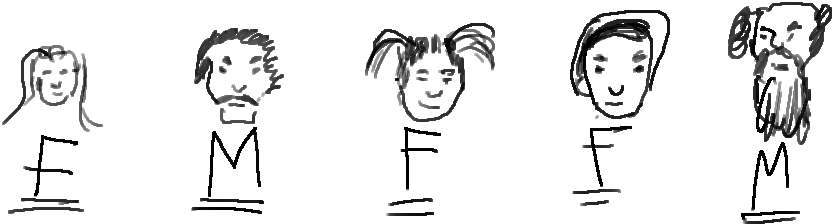
\includegraphics[scale=0.25]{images/classifiedFaces.jpg}
 \pitem Ask computer: Is 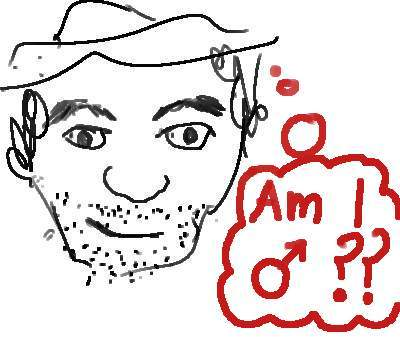
\includegraphics[scale=0.125]{images/maleFace.jpg} a female face?
 \pitem Computer wins if it succeeds with good probability.
\end{itemize}
\end{frame}

\begin{frame}
\frametitle{The binary classification problem formalized}
\begin{itemize}
 \pitem Known set of n features. Eg: Hairstyle, facial hair, moustache present.
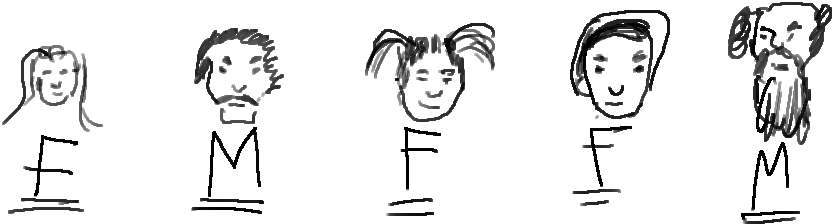
\includegraphics[scale=0.15]{images/classifiedFaces.jpg}
 \pitem Unknown classification function (concept) $c: \set{0,1}^{n} \to \set{M,F}$. Eg: 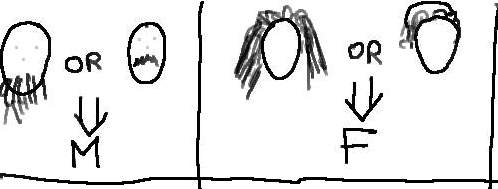
\includegraphics[scale=0.15]{images/concepts.jpg}
 \pitem c belongs to a known set of functions, $C_{n}$. Eg: Polynomial sized DNF over n variables, Halfspaces etc.. 
\pitem See m(n) examples: $\set{(s_{1}, c(s_{1})), (s_{2}, c(s_{2})) .. } = (S, c(S))$.
 \pitem Now, classify test set: $\set{s'_{1}, s'_{2}, ..}$. 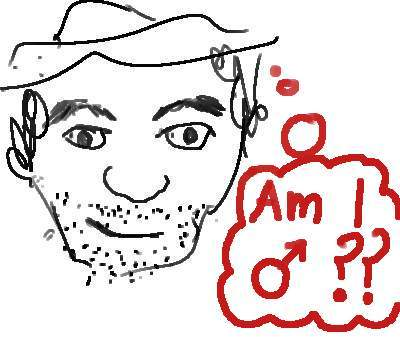
\includegraphics[scale=0.065]{images/maleFace.jpg}
\end{itemize}
\end{frame}

\begin{frame}
\frametitle{Some notation}
\begin{itemize}
\pitem $C_{n}$: a set of classifiction functions $\set{0, 1}^{n} \to \set{0, 1}$. Their ensemble $C = \set{C_{n}}$.
\pitem $D_{n}$: A distribution over inputs: $\set{0,1}^{n}$. Their ensemble: $D = \set{D_{i}}$.\\
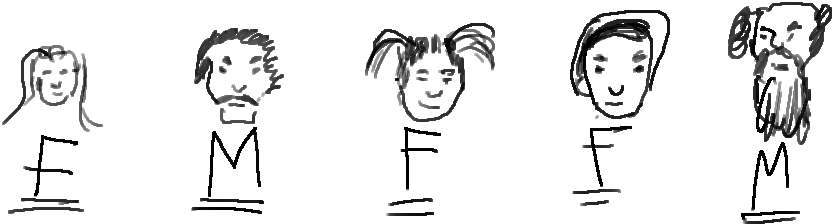
\includegraphics[scale=0.15]{images/classifiedFaces.jpg}
\end{itemize}
\end{frame}

\begin{frame}
\frametitle{L learns a set of functions C wrt D}
\begin{itemize}
\pitem Fix some $c \in C_{n}$. 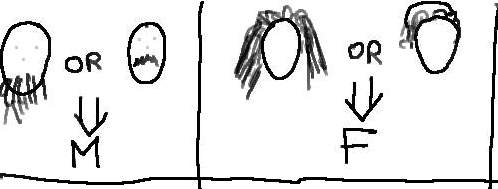
\includegraphics[scale=0.15]{images/concepts.jpg}
\pitem Pick $S \distr D_{n}^{m(n)}$. 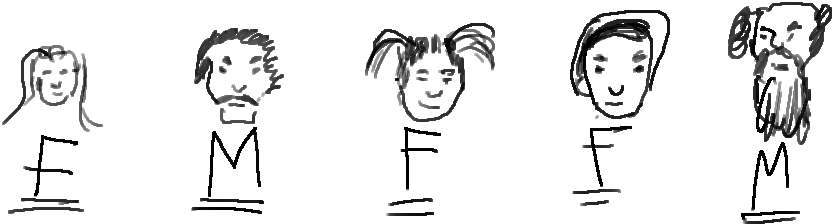
\includegraphics[scale=0.15]{images/classifiedFaces.jpg}
\pitem Alg L, upon studying (S, c(S)) in time $poly(n, \frac{1}{\eps})$, classifies new examples with $\leq \eps$ error rate.
\pitem $$Pr_{S \distr D_{n}^{m(n)}, x \distr D_{n}}(L(S, c(S), x) = c(x)) \geq 1 - \eps$$ in time $poly(n, \frac{1}{\eps})$.
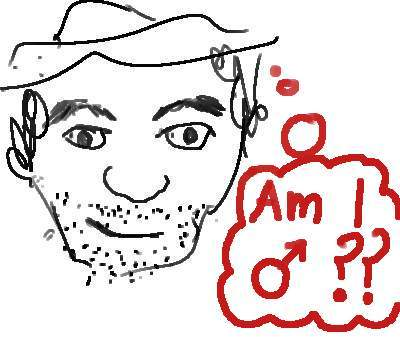
\includegraphics[scale=0.065]{images/maleFace.jpg}
\pitem L learns C if you can say this $\forall c \in C_{n}, D_{n}, \forall n$.
\pitem Else hard to learn.
\end{itemize}
\end{frame}

\begin{frame}
\frametitle{About computational learning theory}
\begin{itemize}
\pitem Can you learn it in polynomial time?
\pitem Is it hard to learn it in polynomial time?
\end{itemize}
\end{frame}

\section{Hardness of learning as a cryptographic assumption}
\subsection{What do we really mean?}
\begin{frame}
\frametitle{Some notation}
\begin{itemize}
\pitem $C_{n}$: a set of classifiction functions $\set{0, 1}^{n} \to \set{0, 1}$.
\pitem $P_{n}$: A distribution over $C_{n}$. Their ensemble: $P = \set{P_{n}}$. 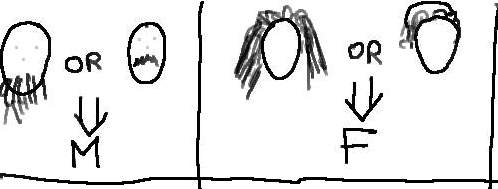
\includegraphics[scale=0.15]{images/concepts.jpg}
\pitem $D_{n}$: A distribution over inputs: $\set{0,1}^{n}$. Their ensemble: $D = \set{D_{i}}$.\\
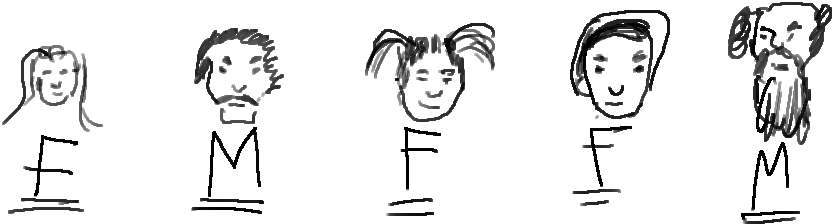
\includegraphics[scale=0.15]{images/classifiedFaces.jpg}
\end{itemize}
\end{frame}

\begin{frame}
\frametitle{Hardness of learning as a cryptographic assumption}
\begin{itemize}
\pitem Want 'C is hard to learn' to be a cryptographic assumption.
\pitem Any alg L should learn C only with negligible probability.
\pitem Take $(P_{n}, D_{n})$. Pick classifier c using $P_{n}$. Pick many examples using $D_{n}$. Your alg cannot match c(x) with non negligible probability.
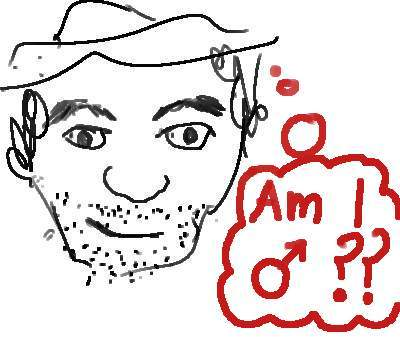
\includegraphics[scale=0.065]{images/maleFace.jpg}
\end{itemize}
\end{frame}

\subsection{A problem in hardness definition}
\begin{frame}
\frametitle{Problem in hardness definition}
\begin{itemize}
\pitem Even if you have efficient alg L to learn all but a tiny scattered subset of C, it is no good. C is 'hard to learn'.\\
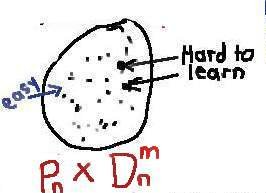
\includegraphics[scale=0.25]{images/hardToLearnDefnProb.jpg}
\pitem If 'Learning C is hard' were a cryptographic assumption, any proof of security built on this assumption would be \textbf{worthless}. L is strong enough to break this assumption, by cryptographic standards.
\end{itemize}
\end{frame}

\subsection{A new definition for hardness of learning}
\begin{frame}
\frametitle{Learning a concept class C wrt $(P, D)$}
\begin{itemize}
\pitem So, weaken hardness of learning defn or strengthen learnability defn.
\pitem Pick $D_{n} \in D, P_{n} \in P, c \in P_{n}$.\\ 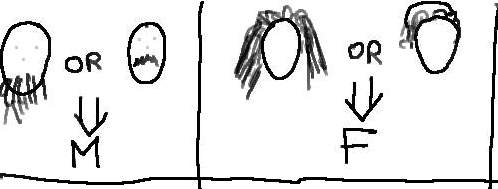
\includegraphics[scale=0.15]{images/concepts.jpg}.......................
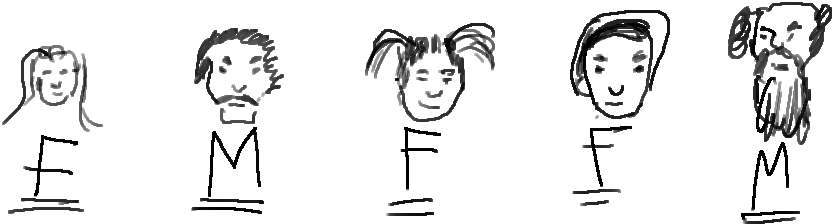
\includegraphics[scale=0.15]{images/classifiedFaces.jpg}
\pitem Alg L, upon studying S, c(S) in time $poly(n, \frac{1}{\eps})$, classifies new examples with $\leq \eps$ error rate.
\pitem $$Pr_{S \distr D_{n}^{m(n)}, x \distr D_{n}, \red{c \in P_{n}}}(L(S, c(S), x) = c(x)) \geq 1 - \eps$$.
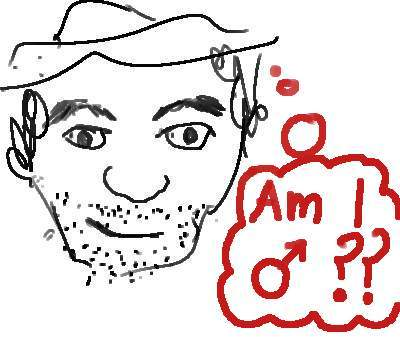
\includegraphics[scale=0.065]{images/maleFace.jpg}
\pitem L learns C if you can say this $\forall P_{n}, D_{n}$.
\pitem Else hard to learn.
\end{itemize}
\end{frame}

\begin{frame}
\frametitle{The new defintion, pictorially}
'Hard to learn': 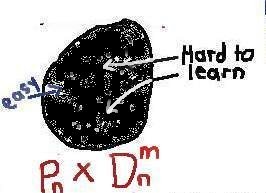
\includegraphics[scale=0.25]{images/hardToLearnDefnNew.jpg}\\
'Learnable': 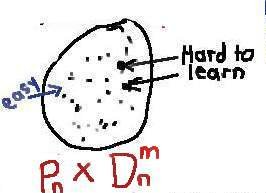
\includegraphics[scale=0.25]{images/hardToLearnDefnProb.jpg}
\end{frame}

\section{Pseudorandom generator from Hard to learn set of functions}
\begin{frame}
\frametitle{Pseudorandom bit generator (PRBG)}
\begin{itemize}
\pitem $G_{n}$ takes n bits input, makes $g(n)>n$ bits output.
\pitem Any polynomial time alg T does not behave noticably differently on $y \distr U(\set{0, 1}^{g(n)})$ and $g(x)| x \distr U(\set{0, 1}^{n})$.
\pitem $G = \set{G_{n}}$.
\pitem Now, construct a PRBG.
\end{itemize}
\end{frame}

\begin{frame}
\frametitle{Construct PRBG from hard to learn $P_{n}$ over $C_{n}$}
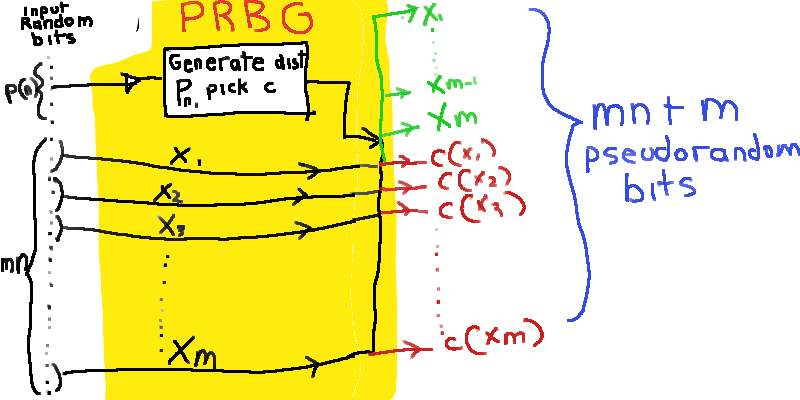
\includegraphics[scale=0.3]{images/prbg.jpg}
\begin{itemize}
\pitem Proof by contradiction: If you could break this PRBG, $C_{n}$ not hard to learn wrt $(P_{n}, U(\set{0, 1}^{n})$.
\item 1110011100111100001011001... \textit{'Can I predict the next bit?'}
\end{itemize}
\end{frame}

% \begin{frame}
% \frametitle{}
% \begin{itemize}
% \pitem 
% \end{itemize}
% \end{frame}

\section{Conclusion}
\begin{frame}
\frametitle{Some other results in the paper: Skip}
\begin{itemize}
\pitem Things you can make from hard to learn set of functions:
One way functions, A private key cryptosystem.
\pitem A pseudo random generator based on hardness of learning parity functions in the presence of noise.
\pitem They take more pains to relate the circuit size and depth required to evaluate functions in hard to learn $C_{n}$ with the circuit depth and size of the primitives generated.
\end{itemize}
\end{frame}

\begin{frame}
\frametitle{The take home message}
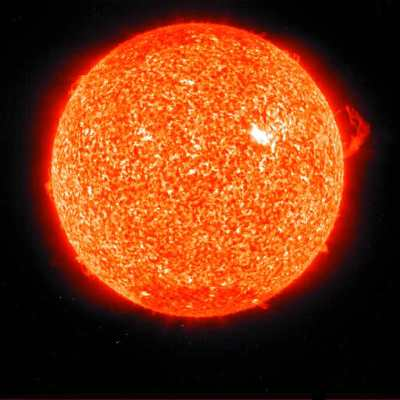
\includegraphics[scale=.25]{images/sun.jpg}
\begin{itemize}
\pitem Can use hardness of learning, properly defined, as a cryptographic assumption.
\pitem Can generically make pseudorandom bit generator from hard to learn but easy to evaluate classes of functions.
\end{itemize}
\end{frame}

\begin{frame}
\frametitle{Bye!}
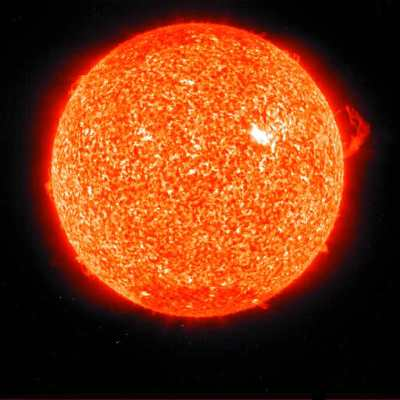
\includegraphics[scale=.5]{images/sun.jpg}
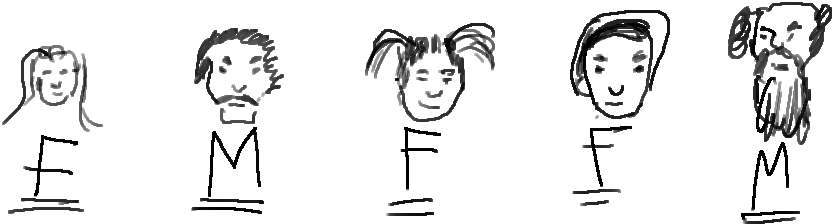
\includegraphics[scale=0.25]{images/classifiedFaces.jpg}
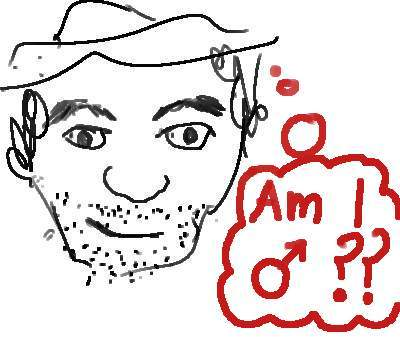
\includegraphics[scale=0.065]{images/maleFace.jpg}
\end{frame}

% \bibliographystyle{plain}
% \bibliography{../}


\end{document}
